%% bare_conf.tex
%% V1.3
%% 2007/01/11
%% by Michael Shell
%% See:
%% http://www.michaelshell.org/
%% for current contact information.
%%
%% This is a skeleton file demonstrating the use of IEEEtran.cls
%% (requires IEEEtran.cls version 1.7 or later) with an IEEE conference paper.
%%
%% Support sites:
%% http://www.michaelshell.org/tex/ieeetran/
%% http://www.ctan.org/tex-archive/macros/latex/contrib/IEEEtran/
%% and
%% http://www.ieee.org/

%%*************************************************************************
%% Legal Notice:
%% This code is offered as-is without any warranty either expressed or
%% implied; without even the implied warranty of MERCHANTABILITY or
%% FITNESS FOR A PARTICULAR PURPOSE! 
%% User assumes all risk.
%% In no event shall IEEE or any contributor to this code be liable for
%% any damages or losses, including, but not limited to, incidental,
%% consequential, or any other damages, resulting from the use or misuse
%% of any information contained here.
%%
%% All comments are the opinions of their respective authors and are not
%% necessarily endorsed by the IEEE.
%%
%% This work is distributed under the LaTeX Project Public License (LPPL)
%% ( http://www.latex-project.org/ ) version 1.3, and may be freely used,
%% distributed and modified. A copy of the LPPL, version 1.3, is included
%% in the base LaTeX documentation of all distributions of LaTeX released
%% 2003/12/01 or later.
%% Retain all contribution notices and credits.
%% ** Modified files should be clearly indicated as such, including  **
%% ** renaming them and changing author support contact information. **
%%
%% File list of work: IEEEtran.cls, IEEEtran_HOWTO.pdf, bare_adv.tex,
%%                    bare_conf.tex, bare_jrnl.tex, bare_jrnl_compsoc.tex
%%*************************************************************************

% *** Authors should verify (and, if needed, correct) their LaTeX system  ***
% *** with the testflow diagnostic prior to trusting their LaTeX platform ***
% *** with production work. IEEE's font choices can trigger bugs that do  ***
% *** not appear when using other class files.                            ***
% The testflow support page is at:
% http://www.michaelshell.org/tex/testflow/


% Note that the a4paper option is mainly intended so that authors in
% countries using A4 can easily print to A4 and see how their papers will
% look in print - the typesetting of the document will not typically be
% affected with changes in paper size (but the bottom and side margins will).
% Use the testflow package mentioned above to verify correct handling of
% both paper sizes by the user's LaTeX system.
%
% Also note that the "draftcls" or "draftclsnofoot", not "draft", option
% should be used if it is desired that the figures are to be displayed in
% draft mode.
%
\documentclass[conference, letterpaper]{IEEEtran}
% Add the compsoc option for Computer Society conferences.
%
% If IEEEtran.cls has not been installed into the LaTeX system files,
% manually specify the path to it like:
% \documentclass[conference]{../sty/IEEEtran}





% Some very useful LaTeX packages include:
% (uncomment the ones you want to load)


% *** MISC UTILITY PACKAGES ***
%
%\usepackage{ifpdf}
% Heiko Oberdiek's ifpdf.sty is very useful if you need conditional
% compilation based on whether the output is pdf or dvi.
% usage:
% \ifpdf
%   % pdf code
% \else
%   % dvi code
% \fi
% The latest version of ifpdf.sty can be obtained from:
% http://www.ctan.org/tex-archive/macros/latex/contrib/oberdiek/
% Also, note that IEEEtran.cls V1.7 and later provides a builtin
% \ifCLASSINFOpdf conditional that works the same way.
% When switching from latex to pdflatex and vice-versa, the compiler may
% have to be run twice to clear warning/error messages.






% *** CITATION PACKAGES ***
%
%\usepackage{cite}
% cite.sty was written by Donald Arseneau
% V1.6 and later of IEEEtran pre-defines the format of the cite.sty package
% \cite{} output to follow that of IEEE. Loading the cite package will
% result in citation numbers being automatically sorted and properly
% "compressed/ranged". e.g., [1], [9], [2], [7], [5], [6] without using
% cite.sty will become [1], [2], [5]--[7], [9] using cite.sty. cite.sty's
% \cite will automatically add leading space, if needed. Use cite.sty's
% noadjust option (cite.sty V3.8 and later) if you want to turn this off.
% cite.sty is already installed on most LaTeX systems. Be sure and use
% version 4.0 (2003-05-27) and later if using hyperref.sty. cite.sty does
% not currently provide for hyperlinked citations.
% The latest version can be obtained at:
% http://www.ctan.org/tex-archive/macros/latex/contrib/cite/
% The documentation is contained in the cite.sty file itself.






% *** GRAPHICS RELATED PACKAGES ***
%
\ifCLASSINFOpdf
  % \usepackage[pdftex]{graphicx}
  % declare the path(s) where your graphic files are
  % \graphicspath{{../pdf/}{../jpeg/}}
  % and their extensions so you won't have to specify these with
  % every instance of \includegraphics
  % \DeclareGraphicsExtensions{.pdf,.jpeg,.png}
\else
  % or other class option (dvipsone, dvipdf, if not using dvips). graphicx
  % will default to the driver specified in the system graphics.cfg if no
  % driver is specified.
  % \usepackage[dvips]{graphicx}
  % declare the path(s) where your graphic files are
  % \graphicspath{{../eps/}}
  % and their extensions so you won't have to specify these with
  % every instance of \includegraphics
  % \DeclareGraphicsExtensions{.eps}
\fi
% graphicx was written by David Carlisle and Sebastian Rahtz. It is
% required if you want graphics, photos, etc. graphicx.sty is already
% installed on most LaTeX systems. The latest version and documentation can
% be obtained at: 
% http://www.ctan.org/tex-archive/macros/latex/required/graphics/
% Another good source of documentation is "Using Imported Graphics in
% LaTeX2e" by Keith Reckdahl which can be found as epslatex.ps or
% epslatex.pdf at: http://www.ctan.org/tex-archive/info/
%
% latex, and pdflatex in dvi mode, support graphics in encapsulated
% postscript (.eps) format. pdflatex in pdf mode supports graphics
% in .pdf, .jpeg, .png and .mps (metapost) formats. Users should ensure
% that all non-photo figures use a vector format (.eps, .pdf, .mps) and
% not a bitmapped formats (.jpeg, .png). IEEE frowns on bitmapped formats
% which can result in "jaggedy"/blurry rendering of lines and letters as
% well as large increases in file sizes.
%
% You can find documentation about the pdfTeX application at:
% http://www.tug.org/applications/pdftex





% *** MATH PACKAGES ***
%
%\usepackage[cmex10]{amsmath}
% A popular package from the American Mathematical Society that provides
% many useful and powerful commands for dealing with mathematics. If using
% it, be sure to load this package with the cmex10 option to ensure that
% only type 1 fonts will utilized at all point sizes. Without this option,
% it is possible that some math symbols, particularly those within
% footnotes, will be rendered in bitmap form which will result in a
% document that can not be IEEE Xplore compliant!
%
% Also, note that the amsmath package sets \interdisplaylinepenalty to 10000
% thus preventing page breaks from occurring within multiline equations. Use:
%\interdisplaylinepenalty=2500
% after loading amsmath to restore such page breaks as IEEEtran.cls normally
% does. amsmath.sty is already installed on most LaTeX systems. The latest
% version and documentation can be obtained at:
% http://www.ctan.org/tex-archive/macros/latex/required/amslatex/math/





% *** SPECIALIZED LIST PACKAGES ***
%
%\usepackage{algorithmic}
% algorithmic.sty was written by Peter Williams and Rogerio Brito.
% This package provides an algorithmic environment fo describing algorithms.
% You can use the algorithmic environment in-text or within a figure
% environment to provide for a floating algorithm. Do NOT use the algorithm
% floating environment provided by algorithm.sty (by the same authors) or
% algorithm2e.sty (by Christophe Fiorio) as IEEE does not use dedicated
% algorithm float types and packages that provide these will not provide
% correct IEEE style captions. The latest version and documentation of
% algorithmic.sty can be obtained at:
% http://www.ctan.org/tex-archive/macros/latex/contrib/algorithms/
% There is also a support site at:
% http://algorithms.berlios.de/index.html
% Also of interest may be the (relatively newer and more customizable)
% algorithmicx.sty package by Szasz Janos:
% http://www.ctan.org/tex-archive/macros/latex/contrib/algorithmicx/




% *** ALIGNMENT PACKAGES ***
%
%\usepackage{array}
% Frank Mittelbach's and David Carlisle's array.sty patches and improves
% the standard LaTeX2e array and tabular environments to provide better
% appearance and additional user controls. As the default LaTeX2e table
% generation code is lacking to the point of almost being broken with
% respect to the quality of the end results, all users are strongly
% advised to use an enhanced (at the very least that provided by array.sty)
% set of table tools. array.sty is already installed on most systems. The
% latest version and documentation can be obtained at:
% http://www.ctan.org/tex-archive/macros/latex/required/tools/


%\usepackage{mdwmath}
%\usepackage{mdwtab}
% Also highly recommended is Mark Wooding's extremely powerful MDW tools,
% especially mdwmath.sty and mdwtab.sty which are used to format equations
% and tables, respectively. The MDWtools set is already installed on most
% LaTeX systems. The lastest version and documentation is available at:
% http://www.ctan.org/tex-archive/macros/latex/contrib/mdwtools/


% IEEEtran contains the IEEEeqnarray family of commands that can be used to
% generate multiline equations as well as matrices, tables, etc., of high
% quality.


%\usepackage{eqparbox}
% Also of notable interest is Scott Pakin's eqparbox package for creating
% (automatically sized) equal width boxes - aka "natural width parboxes".
% Available at:
% http://www.ctan.org/tex-archive/macros/latex/contrib/eqparbox/





% *** SUBFIGURE PACKAGES ***
%\usepackage[tight,footnotesize]{subfigure}
% subfigure.sty was written by Steven Douglas Cochran. This package makes it
% easy to put subfigures in your figures. e.g., "Figure 1a and 1b". For IEEE
% work, it is a good idea to load it with the tight package option to reduce
% the amount of white space around the subfigures. subfigure.sty is already
% installed on most LaTeX systems. The latest version and documentation can
% be obtained at:
% http://www.ctan.org/tex-archive/obsolete/macros/latex/contrib/subfigure/
% subfigure.sty has been superceeded by subfig.sty.



%\usepackage[caption=false]{caption}
%\usepackage[font=footnotesize]{subfig}
% subfig.sty, also written by Steven Douglas Cochran, is the modern
% replacement for subfigure.sty. However, subfig.sty requires and
% automatically loads Axel Sommerfeldt's caption.sty which will override
% IEEEtran.cls handling of captions and this will result in nonIEEE style
% figure/table captions. To prevent this problem, be sure and preload
% caption.sty with its "caption=false" package option. This is will preserve
% IEEEtran.cls handing of captions. Version 1.3 (2005/06/28) and later 
% (recommended due to many improvements over 1.2) of subfig.sty supports
% the caption=false option directly:
%\usepackage[caption=false,font=footnotesize]{subfig}
%
% The latest version and documentation can be obtained at:
% http://www.ctan.org/tex-archive/macros/latex/contrib/subfig/
% The latest version and documentation of caption.sty can be obtained at:
% http://www.ctan.org/tex-archive/macros/latex/contrib/caption/




% *** FLOAT PACKAGES ***
%
%\usepackage{fixltx2e}
% fixltx2e, the successor to the earlier fix2col.sty, was written by
% Frank Mittelbach and David Carlisle. This package corrects a few problems
% in the LaTeX2e kernel, the most notable of which is that in current
% LaTeX2e releases, the ordering of single and double column floats is not
% guaranteed to be preserved. Thus, an unpatched LaTeX2e can allow a
% single column figure to be placed prior to an earlier double column
% figure. The latest version and documentation can be found at:
% http://www.ctan.org/tex-archive/macros/latex/base/



%\usepackage{stfloats}
% stfloats.sty was written by Sigitas Tolusis. This package gives LaTeX2e
% the ability to do double column floats at the bottom of the page as well
% as the top. (e.g., "\begin{figure*}[!b]" is not normally possible in
% LaTeX2e). It also provides a command:
%\fnbelowfloat
% to enable the placement of footnotes below bottom floats (the standard
% LaTeX2e kernel puts them above bottom floats). This is an invasive package
% which rewrites many portions of the LaTeX2e float routines. It may not work
% with other packages that modify the LaTeX2e float routines. The latest
% version and documentation can be obtained at:
% http://www.ctan.org/tex-archive/macros/latex/contrib/sttools/
% Documentation is contained in the stfloats.sty comments as well as in the
% presfull.pdf file. Do not use the stfloats baselinefloat ability as IEEE
% does not allow \baselineskip to stretch. Authors submitting work to the
% IEEE should note that IEEE rarely uses double column equations and
% that authors should try to avoid such use. Do not be tempted to use the
% cuted.sty or midfloat.sty packages (also by Sigitas Tolusis) as IEEE does
% not format its papers in such ways.





% *** PDF, URL AND HYPERLINK PACKAGES ***
%
%\usepackage{url}
% url.sty was written by Donald Arseneau. It provides better support for
% handling and breaking URLs. url.sty is already installed on most LaTeX
% systems. The latest version can be obtained at:
% http://www.ctan.org/tex-archive/macros/latex/contrib/misc/
% Read the url.sty source comments for usage information. Basically,
% \url{my_url_here}.





% *** Do not adjust lengths that control margins, column widths, etc. ***
% *** Do not use packages that alter fonts (such as pslatex).         ***
% There should be no need to do such things with IEEEtran.cls V1.6 and later.
% (Unless specifically asked to do so by the journal or conference you plan
% to submit to, of course. )


% correct bad hyphenation here
\hyphenation{op-tical net-works semi-conduc-tor}

\usepackage{subcaption}

% *** GRAPHICS RELATED PACKAGES ***
%
\ifCLASSINFOpdf
   \usepackage[pdftex]{graphicx}
\else
\fi

% *** MATH PACKAGES ***
%
\usepackage[cmex10]{amsmath}
\usepackage{color}
%
\usepackage{fancyhdr}

\renewcommand{\thispagestyle}[2]{} 


\fancypagestyle{plain}{
        \fancyhead{}
        \fancyhead[C]{first page center header}
        \fancyfoot{}
        \fancyfoot[C]{first page center footer}
}
\pagestyle{fancy}


\headheight 20pt
\footskip 20pt

\rhead{}

%Enter the first page number of your paper below
\setcounter{page}{1}

%Header
\fancyhead[R]{\textit{Science and Information Conference 2014 \\ August 27-29, 2014 $|$ London, UK}}
\renewcommand{\headrulewidth}{0pt}

%Footer
\fancyfoot[C]{www.conference.thesai.org}
\renewcommand{\footrulewidth}{0.5pt}
\fancyfoot[R]{\thepage \  $|$ P a g e }


\begin{document}

%
% paper title
% can use linebreaks \\ within to get better formatting as desired
\title{Developing Software Center Using Evolutionary Prototyping Based-on HTML5}


% author names and affiliations
% use a multiple column layout for up to three different
% affiliations
\author{\IEEEauthorblockN{Imam Riadi}
\IEEEauthorblockA{Information Systems Study Program, Faculty of\\
Mathematics and Natural Sciences,\\
Ahmad Dahlan University, Yogyakarta, Indonesia}
\and
\IEEEauthorblockN{Estu Fardani}
\IEEEauthorblockA{Informatics Department, Science and Technology Faculty,\\
Sunan Kalijaga State Islamic University,\\
Yogyakarta, Indonesia}}

% conference papers do not typically use \thanks and this command
% is locked out in conference mode. If really needed, such as for
% the acknowledgment of grants, issue a \IEEEoverridecommandlockouts
% after \documentclass

% for over three affiliations, or if they all won't fit within the width
% of the page, use this alternative format:
% 
%\author{\IEEEauthorblockN{Michael Shell\IEEEauthorrefmark{1},
%Homer Simpson\IEEEauthorrefmark{2},
%James Kirk\IEEEauthorrefmark{3}, 
%Montgomery Scott\IEEEauthorrefmark{3} and
%Eldon Tyrell\IEEEauthorrefmark{4}}
%\IEEEauthorblockA{\IEEEauthorrefmark{1}School of Electrical and Computer Engineering\\
%Georgia Institute of Technology,
%Atlanta, Georgia 30332--0250\\ Email: see http://www.michaelshell.org/contact.html}
%\IEEEauthorblockA{\IEEEauthorrefmark{2}Twentieth Century Fox, Springfield, USA\\
%Email: homer@thesimpsons.com}
%\IEEEauthorblockA{\IEEEauthorrefmark{3}Starfleet Academy, San Francisco, California 96678-2391\\
%Telephone: (800) 555--1212, Fax: (888) 555--1212}
%\IEEEauthorblockA{\IEEEauthorrefmark{4}Tyrell Inc., 123 Replicant Street, Los Angeles, California 90210--4321}}

% use for special paper notices
%\IEEEspecialpapernotice{(Invited Paper)}

% make the title area
\maketitle

\begin{abstract}
%\boldmath
The Software Center is a required application in all operating system, both conventional or mobile devices. BlankOn as the local operating system should have this application but in reality this application is not yet available. HTML5 is a trend of programming because this technology easy to adapted for desktop utilization. This research tries to make software center HMTL5-based as solution for BlankOn. System development methods used in this study is evolutionary prototyping. It possible to develop application base on prototype of software. Next step is implement prototype to language programming. Every progress will be correction to get better features. Progress will be finished if prototype had all features what needs. Stages of research is divided into several steps. first analysis similar applications, second design system, third implementation and testing of the system. Based on the results of functionality testing software center, the percentage obtained 100\% agree the system can run well. From the results usability testing software center, it is concluded that the respondents strongly agreed that as much as 80\% and 20\% agree. It can be concluded that the software center application can run well and smoothly.

\emph{Keywords : Vala; Webkit; HTML5; Software Center; BlankOn}
\end{abstract}
% IEEEtran.cls defaults to using nonbold math in the Abstract.
% This preserves the distinction between vectors and scalars. However,
% if the conference you are submitting to favors bold math in the abstract,
% then you can use LaTeX's standard command \boldmath at the very start
% of the abstract to achieve this. Many IEEE journals/conferences frown on
% math in the abstract anyway.

% no keywords


% For peer review papers, you can put extra information on the cover
% page as needed:
% \ifCLASSOPTIONpeerreview
% \begin{center} \bfseries EDICS Category: 3-BBND \end{center}
% \fi
%
% For peerreview papers, this IEEEtran command inserts a page break and
% creates the second title. It will be ignored for other modes.
\IEEEpeerreviewmaketitle

\section{Introduction}
% no \IEEEPARstart
Software Center has a function to management software, which adds, removes and update software. Its existence is necessary in all operating systems both desktop and mobile devices. This application use on OpenSUSE, Ubuntu, Mac OS X, Android, iOS, BlackBerry and Windows. However, these applications are not in BlankOn Linux as Indonesian local Linux distribution. Installation of applications in BlankOn Linux currently can be done in the traditional way: first from the console (terminal), this way can be done if you know the name of the application you want to install the package. The second way to use the Synaptic Package Manager a management application packages. Despite using a GUI (graphic user interface) but still only be done if you know the name of the application you want to install the package and limited its use. Making it difficult for an ordinary user to install the application.

Similar applications that have been there is the Ubuntu Software Center for Ubuntu distribution. This application allowing licensed OpenSource applied to BlankOn Linux. However, since these applications have become a trademark of Ubuntu, needs further modification process. This process takes time and is not guaranteed to run well so, what ideas arise if made ​​to start from scratch.

HTML5 is a trend of programming because this technology easy to adapted, can run in many platforms up to desktop utilization. Manokwari Desktop a desktop environment for BlankOn Linux is base on HTML5 and GNOME 3. Development software center base on HTML5 can run consistent with development of BlankOn Linux [1]. This research tries to make software center HMTL5-based as solution for BlankOn Linux.

% You must have at least 2 lines in the paragraph with the drop letter
% (should never be an issue)
\section{Similar Software Center}

YaST (Yet another Setup Tool)
Software center for openSUSE. It use to manage all of user need for use openSUSE. Example to install application, package, network setting etc. YaST use ruby and YCP for language programming and Qt for user interface[2].

Ubuntu Software Center\\Software management for Ubuntu by Canonical. It is free software written in Python, PyGTK/PyGObject based on GTK+ and the further development of the GNOME application, gnome-app-install.[3][4]

\section{HTML5 App in Desktop}

\subsection{Webkit and WebkitGTK+}
WebKit is a layout engine software component for rendering web pages in web browsers. It powers Apple's Safari web browser and was previously used in Google Chrome web browser. Figure 1 and 2 shows how Webkit work.

WebKit is also used as the basis for the experimental browser included with the Amazon Kindle e-book reader, as well as the default browser in the Apple iOS, Android, BlackBerry 10, and Tizen mobile operating systems. WebKit's C++ application programming interface provides a set of classes to display web content in windows, and implements browser features such as following links when clicked by the user, managing a back-forward list, and managing a history of pages recently visited [5].

\begin{figure}[!t]
\centering
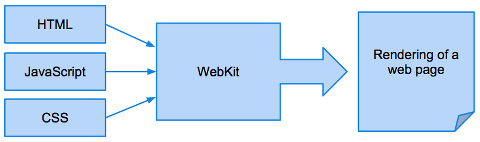
\includegraphics[scale=0.5]{image/webkit.png}
\caption{How Webkit Work}
\end{figure}

\begin{figure}[!t]
\centering
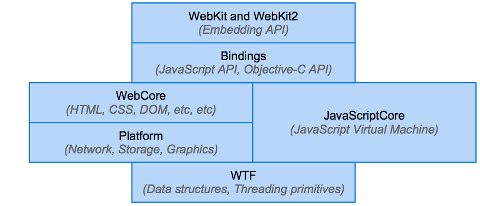
\includegraphics[scale=0.5]{image/webkitcomponents.png}
\caption{Webkit Major Components}
\end{figure}

WebKitGTK+ is the GNOME platform port of the WebKit rendering engine. Offering WebKit’s full functionality through a set of GObject-based APIs, it is suitable for projects requiring any kind of web integration, from hybrid HTML/CSS applications to full-fledged web browsers, like Epiphany and Midori. It’s useful in a wide range of systems from desktop computers to embedded systems like phones, tablets, and televisions. WebKitGTK+ is made by a lively community of developers and designers, who hope to bring the web platform to everyone [6].

\subsection{WarSi (Software Center)}
WarSi (Warung aplikasi) is the name of software center run in BlankOn Linux. It job to help user management applications by make Graphic User Interface. To do management WarSi need link to apt. its use vala programming. Object oriented programming base on c and GObject. 

Valac, the Vala compiler, is a self-hosting compiler that translates Vala source code into C source and header files. It uses the GObject type system to create classes and interfaces declared in the Vala source code. The syntax of Vala is similar to C\#, modified to better fit the GObject type system. Vala supports modern language features as the following: Interfaces; Properties; Signals; Foreach; Lambda; expressions; Type inference for local variables [7].

Vala is designed to allow access to existing C libraries, especially GObject-based libraries, without the need for runtime bindings. All that is needed to use a library with Vala is an API file, containing the class and method declarations in Vala syntax. Vala currently comes with experimental bindings for GLib and GTK+ It's planned to provide generated bindings for the full GNOME Platform at a later stage.

\section{Development WarSi}
\subsection{Design System}

WarSi design base on HTML5, AngularJS for front-end. Back-end use Vala programming. Vala chosen because it can communicate with operating system like run specific apt command use Vala API. Another reason Vala can run simultanly with Manokwari Desktop base on GNOME 3.

Figure 3 show how design of WarSi.

\begin{figure}[!t]
\centering
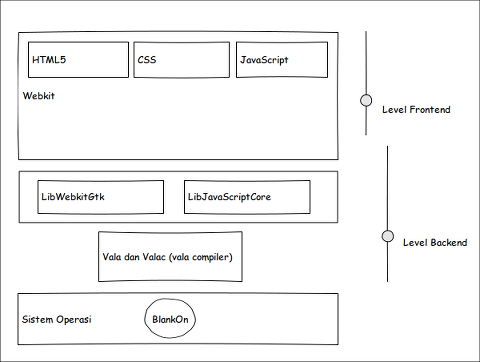
\includegraphics[scale=0.5]{image/DesignSystem.png}
\caption{Design System}
\end{figure}

\subsection{Development Method}
System development methods used in this study is the method of Evolutionary Prototyping. Evolutionary prototyping method has the steps as shown in Figure 4 [8].

\begin{figure}[!t]
\centering
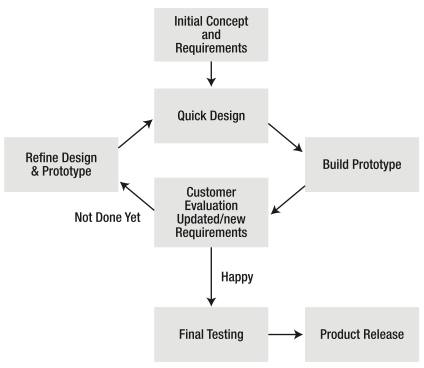
\includegraphics[scale=0.5]{image/ep-model.png}
\caption{Evolutionary Prototyping Process Model}
\end{figure}

Evolutionary prototyping provides other benefits including[9]: the clarification of management and user requirements; the ability to uncover missing or previously unknown requirements; the flexibility to meet changing constraints for software systems; the provision of a method whereby users, management, and developers can communicate about systems; the easing of maintenance tasks; the creation of ‘better’ user interfaces; prototyping with quality; and the ability for developers to reflect on lessons learned during system development.

Steps of Evolutionary Prototyping:
\subsubsection{Initial Concept and Requirement}
At this stage will be determined what will be in software center includes system requirements,  criteria, the function to be achieved. This stage is important that detailed description of the application can be explained from the beginning.

\subsubsection{Quick Design}
The stage design is done in standard applications with minimal functionality to answer the important points that have been described in the previous step. Design prototype mock-up done in the form of the initial design and the functions that can run applications.

\subsubsection{Build Prototype}
From the results of the initial prototype design to be started in the form of program code. Starting from the design of the interface using HTML5, CSS3, javascript. The design is achieved not have to be exactly the same as designed. The next thing is to combine the Vala programming, Webkit as the back-end Software Center. Installation of container is done at this stage that some of the functions of the application can run. After this initial prototype Software Center obtained. This process also includes whether the application can be run
in BlankOn Linux.

\subsubsection{Costumer Evaluation, Update}
Prototype has been done early discussion back to the client for review and evaluate, both design, functional, and usability. Any corrections and recommendation will be collected.

\subsubsection{If not done yet, Refine design and prototype}
If client not satisfied, prototype must be correction base on recommendation which have been collect in previously.

\subsubsection{If happy, final testing and product release}
Once the prototype is approved client, the application entered the stage of release and make documentation of software center. 

\subsection{UML (Unified Modelling Language}

\subsubsection{Use Case Diagram}
Figure 5 show the use case diagram for software center.

\begin{figure}[!t]
\centering
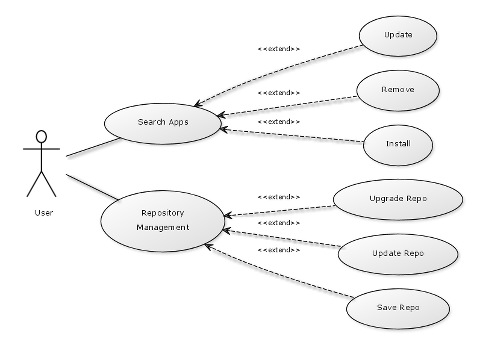
\includegraphics[scale=0.42]{image/Usecase.png}
\caption{Use case Diagram}
\end{figure}

This is a description of the process in the use case diagram:
\begin{itemize}
\item Search Application\\
This process is performed to find the application as the user desires. Once the search is complete the user can install / remove applications and application upgrades.
\item Repository Management\\
This funtions make user can change source repository, save, update and upgrade system.
\end{itemize}

\subsubsection{Activity Diagram}
Figure 6 show activity diagram generally.

\begin{figure}[!t]
\centering
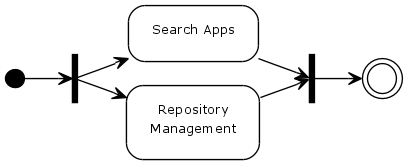
\includegraphics[scale=0.7]{image/ActivityDiagram.png}
\caption{Activity Diagram}
\end{figure}

\begin{figure}[!t]
\centering
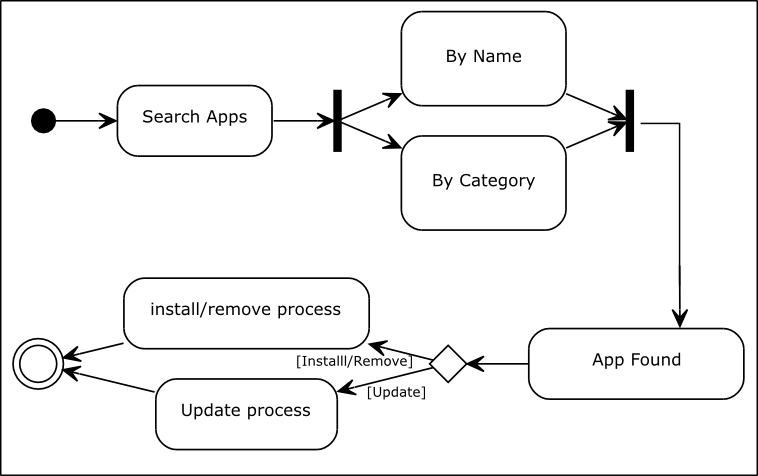
\includegraphics[scale=0.5]{image/ADSearchApp.png}
\caption{Activity Diagram Search Application}
\end{figure}

Activity Diagram Search Applications. Figure 7 is an activity diagram for a search application. Search Application is divided into two, namely by entering a keyword in the search field and the search for applications by category. Process for Figure 7 are:
\begin{itemize}
\item Users select search for applications by name or by category of applications,
\item If you select by name, users enter a keyword or the name of the application you are looking for in the search field to find the application,
\item If you select a category based application, the user selects a category that existed until the application is found,
\item Application is found, the user chose to install/remove or update the application,
\item Installation process, and the process is complete.
\end{itemize}

Activity Diagram Repository Management. Process for Figure 8 are:
\begin{itemize}
\item User select a menu from the main menu next repository, system will display the page repository, there are two options, choose source repository or directly perform the update,
\item User can make changes to the repository by selecting the list
repository that is already available,
\item When the user makes changes to the repository, the system will saved the changes,
\item When the user performs an update to the update repository the repository will be made and the system will display the process update,
\item After update user can upgrade system if available, then the system will display the process upgrade.
\item Process is completed.
\end{itemize}

\begin{figure}[!t]
\centering
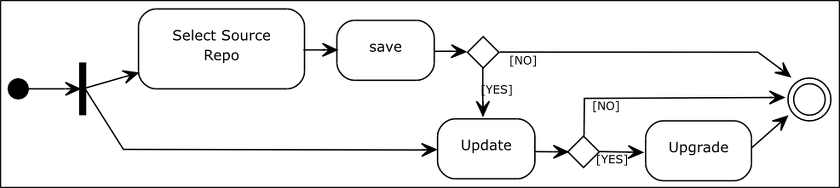
\includegraphics[scale=0.5]{image/ADManagement.png}
\caption{Activity Diagram Repository Management}
\end{figure}

\subsubsection{Sequence Diagram}
Figure 9 show sequence diagram for search application by name.

\begin{figure}[!t]
\centering
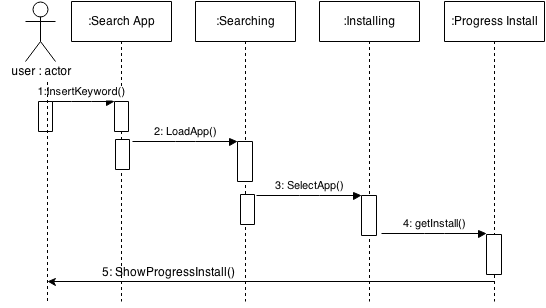
\includegraphics[scale=0.4]{image/SearchbyName.png}
\caption{Sequence Diagram Search Application by Name}
\end{figure}

\begin{figure}[!t]
\centering
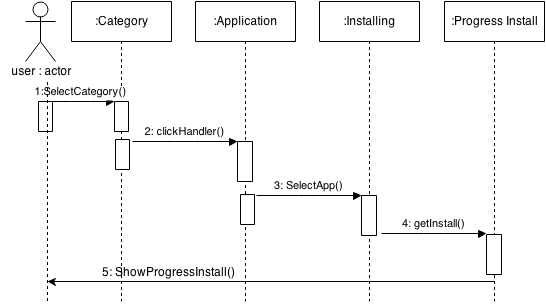
\includegraphics[scale=0.4]{image/SearchbyCategory.png}
\caption{Sequence Diagram Search Application by Category}
\end{figure}

\begin{figure}[!t]
\centering
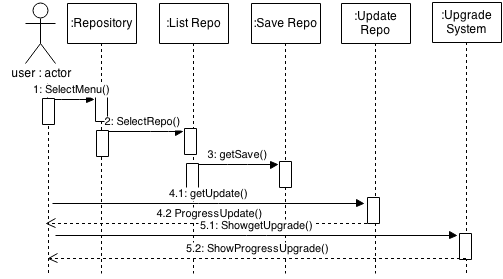
\includegraphics[scale=0.4]{image/ManagementRepo.png}
\caption{Sequence Diagram Management Repository}
\end{figure}

\subsection{Result Development}
After development finished, the result is prototype software center for BlankOn Linux. Base on HTML5 for front-end. Screenshoot WarSi can be found in Figure 12 and Figure 13.

Figure 14 show page to search application.
\begin{figure}[!t]
\centering
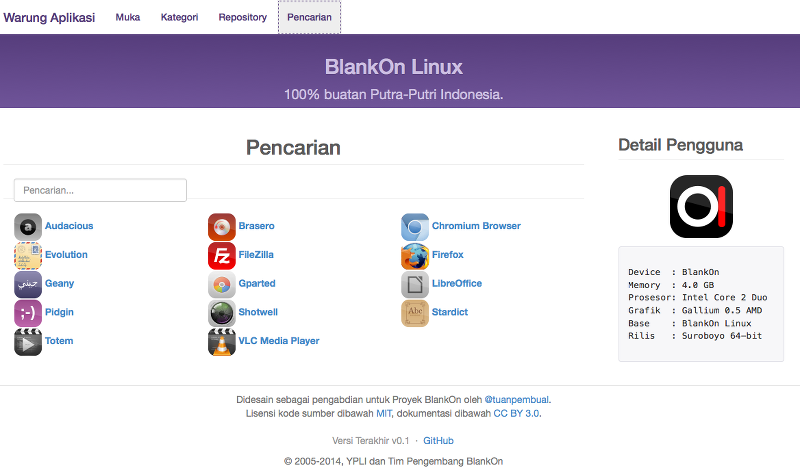
\includegraphics[scale=0.31]{image/03HamalanPencarian.png}
\caption{Implement Search Page}
\end{figure}

Figure 15 show page repository management.
\begin{figure}[!t]
\centering
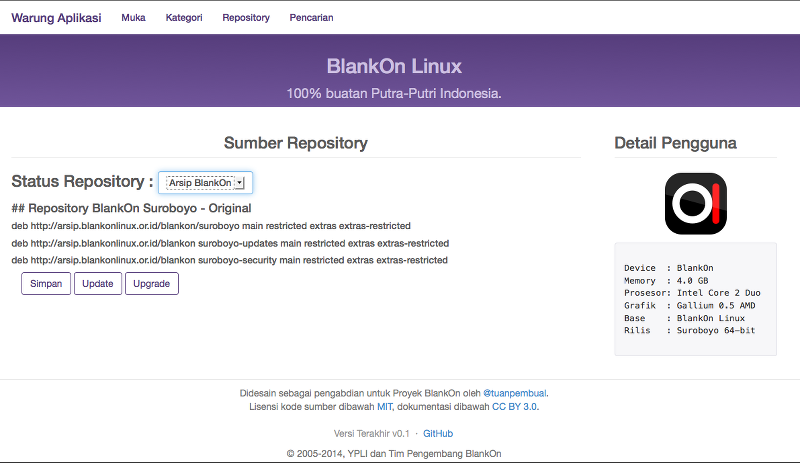
\includegraphics[scale=0.31]{image/02HalamanRepository.png}
\caption{Implement Repository Management}
\end{figure}

\subsection{Testing}
Black box testing (also called functional testing) is testing that ignores the internal mechanism of a system or component and focuses solely on the outputs generated in response to selected inputs and execution conditions.[10]

With black box testing, the software tester does not (or should not) have access to the source code itself. The code is considered to be a “big black box” to the tester who cannot see inside the box. The tester knows only that information can be input into to the black box, and the black box will send something back out.

Parameter testing functionally of WarSI include: can it run?; can it install application; can it remove application; can it search application base on name; can it search application base on category; can it change source repository and save it; can it update and upgrade system. Parameter testing usability of WarSi include: can user use it without trouble (easy to use); will user use it again; how about interface; are users be helped with this application to repository management. 

WarSi tested to 15 random correspondents. Table I and Table II show the result of functionally and usability system.

\begin{table}[!t]
\renewcommand{\arraystretch}{1.3}
\caption{Result Functionally of Testing WarSi}
\label{table_functional}
\centering
\begin{tabular}{|c|c|c|}
\hline
\textbf{Parameter} & \textbf{Yes} & \textbf{No}\\
\hline
WarSi run & 15 & 0\\
\hline
Can install application & 15 & 0\\
\hline
Can remove application & 15 & 0\\
\hline
Can search application by name & 15 & 0\\
\hline
Can search application by category & 15 & 0\\
\hline
Can change repository source & 15 & 0\\
\hline
Can update and upgrade system & 15 & 0\\
\hline
\end{tabular}
\end{table}

\begin{table}[!t]
\renewcommand{\arraystretch}{1.3}
\caption{Result Usability of Testing WarSi}
\label{table_usability}
\centering
\begin{tabular}{|c|c|c|c|c|c|}
\hline
\textbf{Parameter} & \textbf{VA} & \textbf{A} & \textbf{N} & \textbf{D} & \textbf{VD}\\
\hline
WarSi easy to use & 15 & 0 & 0 & 0 & 0\\
\hline
Will use WarSi again & 9 & 6 & 0 & 0 & 0\\
\hline
Graphic User Interface interactive & 10 & 5 & 0 & 0 & 0\\
\hline
WarSi helped to software management & 10 & 5 & 0 & 0 & 0\\
\hline
\end{tabular}
\begin{tabular}{lll}
Notes: &VA=Very Agree& A=Agree;\\
N=Neutral; &D=Disagree; &VD=Very Disagree\\
\end{tabular}
\end{table}

Percentage result functional WarSi:
\begin{itemize}
\item Yes : (75/75) x 100 = 100\%,
\item No : (75/75) x 100 = 0\%,
\end{itemize}

Percentage result usability WarSi:
\begin{itemize}
\item Very Agree : (44/60) x 100 = 73\%,
\item Agree : (16/60 x 100 = 27\%,
\item Neutral : (0/60) x 100 = 0\%,
\item Disagree : (0/60) x 100 = 0\%,
\item Very Disagree : (0/60) x 100 = 0\%,
\end{itemize}

Based on test results involving 15 users, the most of the them give good score to WarSi center software, then the obtained test results showing that 10\% of users say functionality of the system has been running well and 0\% respondents expressed a functional system is not running properly. 

Under the terms of usability testing software center, it is concluded that the majority of respondents are satisfied with the application made. Data usability test results that the respondents strongly agreed by 80\%, 20\% agree, neutral 0\%, which is expressed as 0\% disagree and strongly disagree that states as much as 0\%. Based on these test results, it can be concluded that the software center that has made this feasible for use. However, the need for further development of the application to obtain optimal application. Figure 15 and Figure 16 show percent of functionally and satisfied user using WarSi.

\begin{figure}[!t]
\centering
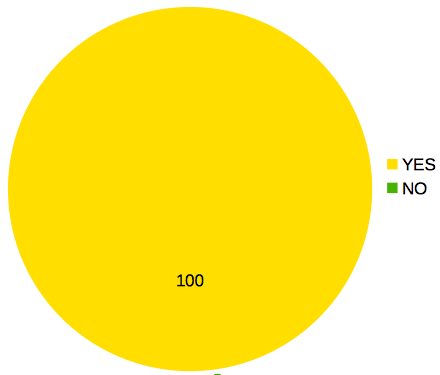
\includegraphics[scale=0.5]{image/functionally.png}
\caption{Result Functionally Testing}
\end{figure}

\begin{figure}[!t]
\centering
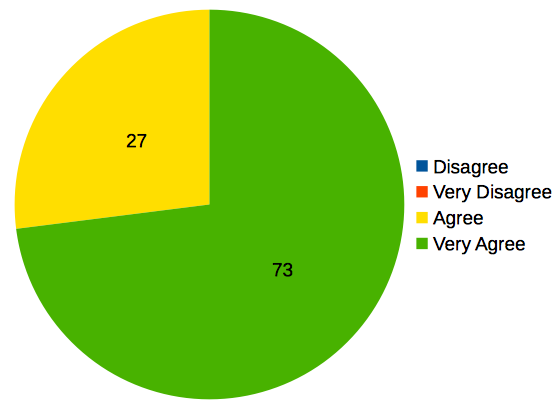
\includegraphics[scale=0.4]{image/usability.png}
\caption{Result Usability Testing}
\end{figure}


% An example of a floating figure using the graphicx package.
% Note that \label must occur AFTER (or within) \caption.
% For figures, \caption should occur after the \includegraphics.
% Note that IEEEtran v1.7 and later has special internal code that
% is designed to preserve the operation of \label within \caption
% even when the captionsoff option is in effect. However, because
% of issues like this, it may be the safest practice to put all your
% \label just after \caption rather than within \caption{}.
%
% Reminder: the "draftcls" or "draftclsnofoot", not "draft", class
% option should be used if it is desired that the figures are to be
% displayed while in draft mode.
%
%\begin{figure}[!t]
%\centering
%\includegraphics[width=2.5in]{myfigure}
% where an .eps filename suffix will be assumed under latex, 
% and a .pdf suffix will be assumed for pdflatex; or what has been declared
% via \DeclareGraphicsExtensions.
%\caption{Simulation Results}
%\label{fig_sim}
%\end{figure}

% Note that IEEE typically puts floats only at the top, even when this
% results in a large percentage of a column being occupied by floats.


% An example of a double column floating figure using two subfigures.
% (The subfig.sty package must be loaded for this to work.)
% The subfigure \label commands are set within each subfloat command, the
% \label for the overall figure must come after \caption.
% \hfil must be used as a separator to get equal spacing.
% The subfigure.sty package works much the same way, except \subfigure is
% used instead of \subfloat.
%
%\begin{figure*}[!t]
%\centerline{\subfloat[Case I]\includegraphics[width=2.5in]{subfigcase1}%
%\label{fig_first_case}}
%\hfil
%\subfloat[Case II]{\includegraphics[width=2.5in]{subfigcase2}%
%\label{fig_second_case}}}
%\caption{Simulation results}
%\label{fig_sim}
%\end{figure*}
%
% Note that often IEEE papers with subfigures do not employ subfigure
% captions (using the optional argument to \subfloat), but instead will
% reference/describe all of them (a), (b), etc., within the main caption.


% An example of a floating table. Note that, for IEEE style tables, the 
% \caption command should come BEFORE the table. Table text will default to
% \footnotesize as IEEE normally uses this smaller font for tables.
% The \label must come after \caption as always.
%
%\begin{table}[!t]
%% increase table row spacing, adjust to taste
%\renewcommand{\arraystretch}{1.3}
% if using array.sty, it might be a good idea to tweak the value of
% \extrarowheight as needed to properly center the text within the cells
%\caption{An Example of a Table}
%\label{table_example}
%\centering
%% Some packages, such as MDW tools, offer better commands for making tables
%% than the plain LaTeX2e tabular which is used here.
%\begin{tabular}{|c||c|}
%\hline
%One & Two\\
%\hline
%Three & Four\\
%\hline
%\end{tabular}
%\end{table}

% Note that IEEE does not put floats in the very first column - or typically
% anywhere on the first page for that matter. Also, in-text middle ("here")
% positioning is not used. Most IEEE journals/conferences use top floats
% exclusively. Note that, LaTeX2e, unlike IEEE journals/conferences, places
% footnotes above bottom floats. This can be corrected via the \fnbelowfloat
% command of the stfloats package.

\section{Conclusion}
Based on the research that have been carried out during development Software Center using Evolutionary Prototyping HTML5-based, it can be concluded as follows:
\begin{itemize}
\item Analysis and development Software Center that can help users to manage applications in BlankOn Linux has been successfully carried out,
\item In this study the HTML5 programming language can be used for development desktop application,
\item Based on the test results showed that the Software Center can be run on BlankOn Linux.
\end{itemize}.

% conference papers do not normally have an appendix

% use section* for acknowledgement
% \section*{Acknowledgment}
% Thank you to Ahmad Dahlan University for funding this research

% trigger a \newpage just before the given reference
% number - used to balance the columns on the last page
% adjust value as needed - may need to be readjusted if
% the document is modified later
%\IEEEtriggeratref{8}
% The "triggered" command can be changed if desired:
%\IEEEtriggercmd{\enlargethispage{-5in}}

% references section

% can use a bibliography generated by BibTeX as a .bbl file
% BibTeX documentation can be easily obtained at:
% http://www.ctan.org/tex-archive/biblio/bibtex/contrib/doc/
% The IEEEtran BibTeX style support page is at:
% http://www.michaelshell.org/tex/ieeetran/bibtex/
%\bibliographystyle{IEEEtran}
% argument is your BibTeX string definitions and bibliography database(s)
%\bibliography{IEEEabrv,../bib/paper}
%
% <OR> manually copy in the resultant .bbl file
% set second argument of \begin to the number of references
% (used to reserve space for the reference number labels box)
\begin{thebibliography}
{1}
% \bibitem{IEEEhowto:kopka}
% H.~Kopka and P.~W. Daly, \emph{A Guide to \LaTeX}, 3rd~ed.\hskip 1em plus
%  0.5em minus 0.4em\relax Harlow, England: Addison-Wesley, 1999.

\bibitem{IEEEhowto:manokwari}
\emph{Manokwari, Desktop shell for GNOME 3 with Gtk+ and HTML5 frontend} available at http://manokwari.blankonlinux.or.id/

\bibitem{IEEEhowto:mac-vicar}
Duncan Mac-Vicar P., \emph{What you should know about YaST}, Novell, Inc, 2008.

\bibitem{IEEEhowto:paul thomas}
Mathew Paul Thomas, \emph{Ubuntu Software Center}, http://wiki.ubuntu.com/SoftwareCenter, 2005.

\bibitem{IEEEhowto:ubuntu}
\emph{Ubuntu Software Center} available at https://launchpad.net/software-center

\bibitem{IEEEhowto:webkit}
Adam Bart, \emph{How WebKit Works}, webkit.org, 2010.

\bibitem{IEEEhowto:webkitgtk}
\emph{WebkitGTK+} available at http://webkitgtk.org/

\bibitem{IEEEhowto:vala}
Muhammad Anwari, \emph{GNOME 3 Application Development Beginner}, Birmingham: Packt Publishing Ltd, 2013.

\bibitem{IEEEhowto:dooley}
John Dooley, \emph{Software Development and Professional Practice}, Springer Science Business Media, Inc, 2011.

\bibitem{IEEEhowto:ryan}
Ryan A. Carter, Annie I. Antón, Aldo Dagnino, Laurie Williams, \emph{Evolving Beyond Requirements Creep:A Risk-Based Evolutionary Prototyping Model}, North Carolina State University, 2001.

\bibitem{IEEEhowto:IEEE}
IEEE, \emph{IEEE Standard 610.12-1990, IEEE Standard Glossary of Software Engineering Terminology}, 1990.

\bibitem{IEEEhowto:williams}
Laurie Williams, \emph{Testing Overview and Black-Box Testing Techniques}, 2006

\end{thebibliography}

% that's all folks
\end{document}